\chapter{\ifenglish Background Knowledge and Theory\else ทฤษฎีที่เกี่ยวข้อง\fi}
\tolerance = 9999
\overfullrule=0pt

% การทำโครงงาน เริ่มต้นด้วยการศึกษาค้นคว้า ทฤษฎีที่เกี่ยวข้อง หรือ งานวิจัย/โครงงาน ที่เคยมีผู้นำเสนอไว้แล้ว ซึ่งเนื้อหาในบทนี้ก็จะเกี่ยวกับการอธิบายถึงสิ่งที่เกี่ยวข้องกับโครงงาน เพื่อให้ผู้อ่านเข้าใจเนื้อหาในบทถัดๆ ไปได้ง่ายขึ้น
\enskip \enskip \enskip \enskip \enskip Miracle from sky ถูกสร้าง และพัฒนาขึ้นโดยโปรแกรม Unity เป็นหลัก
 ซึ่งก่อนที่ผู้พัฒนาจะเริ่มลงมือสร้างเกมจริงขึ้นมา ผู้พัฒนาได้ศึกษาหาความารู้ในด้านต่างๆที่จำเป็นสำหรับการสร้างเกม  
โดยเนื้อหาในบทนี้จะอธิบายในส่วนของความรู้ ทฤษฎีบทที่เกี่ยวข้อง และหลักการต่างๆที่ผู้พัฒนาได้ศึกษา และนำไปใช้ในการสร้างเกม 
เพื่อให้ผู้ที่เข้ามาอ่านได้เข้าใจหลักการต่างๆในเบื้องต้น และเพื่อให้เข้าใจเนื้อหาในบทถัดๆไปได้ง่ายมากยิ่งขึ้น

\section{พื้นฐาน Unity}
\enskip \enskip \enskip \enskip \enskip Unity เป็น software ที่ถูกออกแบบมาเพื่อใช้สำหรับการพัฒนา software ที่สามารถ
จำลองการทำงานต่างๆได้ เช่น game(ทั้ง 2D และ 3D), การขนส่ง, animation, อุตสาหกรรมยานยนต์ เป็นต้น 
ซึ่งสามารถรองรับได้หลากหลาย platform เช่น PC, iOS, Android เป็นต้น โดยในที่นี้จะขออธิบายในส่วนที่เกี่ยวข้องกับการสร้าง
game 3D เท่านั้น

\enskip \enskip โดยส่วนต่างๆใน Unity ที่สำคัญ และจำเป็นต้องศึกษาสำหรับการสร้างเกม มีดังนี้
\subsection{Scene}
คือ ฉากภายในเกม หรือบริเวณที่เรานำสิ่งต่างๆมาใช้รวมกัน ซึ่ง scene มีได้หลาย scene เช่น scene เริ่มเกม,
 scene จบเกม, scene เมนู เป็นต้น
\subsection{GameObject}
คือ วัตถุ หรือสิ่งต่างๆที่สามารถนำมาใช้แสดงผลภายใน scene ได้ เช่น Model ต่างๆ, ตัวเล่นเสียง,
ตัวเล่น effect, light, terrain เป็นต้น
\subsection{Asset}
คือ GameObject หรือสิ่งต่างๆที่นำเข้ามาใช้งานใน project ของเรา เช่น Model ตัวละคร, เสียง, animation,
script, texture, prefab, terrain เป็นต้น โดย asset เราสามารถซื้อจาก Unity Asset Store ได้ ซึ่งมีทั้ง
ที่แจกฟรี และเสียเงิน โดยราคาขึ้นกับคุณภาพของ asset และความพึงพอใจของผู้ขาย
\subsection{Camera}
คือ กล้องที่ใช้สำหรับการแสดงผลเกมของเราออกมาให้ผู้เล่นเห็นทางจอภาพ โดยสามารถปรับมุมมอง ตำแหน่งต่างของกล้องได้อย่างอิสระ 
สามารถตั้งให้กล้องติดตามตัวผู้เล่นได้ รวมไปถึงใช้ในการทำ cutscene
\subsection{Light}
คือ GameObject ประเภทหนึ่งที่สามารถให้แสงสว่างกับ scene ของเราได้ light ทำให้เกิดเงาของ GameObject 
ซึ่งสามารถไปปรับใช้งานได้หลากหลาย เช่น ทำเวลากลางวัน/กลางคืน, ทำ scene มืดๆที่ทำให้รู้สึกถึงความน่ากลัว เป็นต้น
\subsection{Component}
คือ คุณสมบัติ หรือความสามารถต่างๆที่อยู่ใน GameObject ซึ่งมีหลากหลายคุณสมบัติ และคุณสมบัติแต่ละตัวก็มีความแตกต่างกันไป
โดย component ที่สำคัญมีดังนี้ 

\begin{enumerate}
\item Transform คือ component ที่ใช้ในการควบคุมตำแหน่ง(Position) การหมุน(Rotation) และขนาด(Scale) 
โดยทุก GameObject ต้องมีคุณสมบัตินี้
\item Rigidbody คือ component ที่ใช้ในการจัดการเกี่ยวกับระบบฟิสิกส์ของวัตถุ ไม่ว่าจะเป็น แรง(Force), มวล(Mass), 
การแสดงผลจากแรงโน้มถ่วง(Gravity) และการล็อควัตถุ(Freeze)
\item Collider คือ component ที่ใช้ในการตรวจสอบการชนกันของวัตถุต่างๆภายใน scene นำมาประยุกต์ใช้ได้หลากหลายแบบ
เช่น การคำนวณดาเมจ, การระเบิดของลูกบอลไฟเมื่อชนกับวัตถุต่างๆ, การเก็บไอเทมต่างๆ เป็นต้น
\item Animator คือ component ที่ใช้ในการควบคุมการทำงานของ animation ต่างๆ โดยจะควบคุม และแสดงในรูปของ state machine
\item Particle System คือ component ที่ใช้ในการสร้าง visial effect~\cite{VFX} หรือที่เรียกว่า VFX เช่น เปลวไฟ, สายฟ้า, น้ำ เป็นต้น
\item Volume คือ component ที่ใช้ในการควบคุมการแสดงผลทางหน้าจอ หรือภาพที่เราเห็นผ่านทางกล้อง โดยสามารถปรับบริมาณแสงที่ผ่านกล้อง, 
การเบลอขอบจอภาพ, การเพิ่มมุมแบบ perspective ทำให้ภาพที่เห็นถูกยืด หรือหดลงได้
\end{enumerate}

\subsection{Texture}
คือ รูปภาพพื้นผิวต่างๆ ที่ใช้ในการนำมาเป็นผิวของวัตถุ ช่วยให้วัตถุมีความสมจริงมากขึ้น
\subsection{Material}
คือ เม็ดสี หรือสีที่ใช้ลงสีให้กับวัตถุต่างภายใน scene ไม่จำเป็นต้องเป็นสีล้วน โดยถ้าหากใช้ shader graph
ในการสร้าง material จะทำให้ material ที่ได้มีคุณสมบัติที่กำหนดไว้ได้ เช่น material ที่เรืองแสงได้, 
material ที่มีความมันวาว, material ที่เปลี่ยนรูปร่างได้ เป็นต้น
\subsection{SkyBox}
คือ สิ่งที่ให้เปลี่ยน สี รูปแบบ คุณสมบัติต่างๆของท้องฟ้าภายในเกม เช่น สามารถทำให้ท้องฟ้าเป็นกลางคืน/วันได้,
ทำให้ท้องฟ้ามีก้อนเมฆได้ เป็นต้น
\subsection{Wind Zone}
คือ GameObject ประเภทหนึ่ง ทำหน้าที่ช่วยควบคุมการทำงานของระบบลมภายใน scene ช่วยให้เกมมีความสมจริงมากยิ่งขึ้น
\subsection{Terrain}
คือ GameObject ประเภทหนึ่ง ทำหน้าที่ช่วยควบคุม ปรับแต่งภูมิประเทศ หรือสภาพแวดล้อมของพื้น ให้มีลักษณะตามที่เราต้องการ
เช่น ใช้ทำหลุม, ใช้ทำภูเขา, ใช้ทำพื้นที่ยกระดับ เป็นต้น
\subsection{Prefab}
คือ การนำ GameObject ต่างๆมาประกอบกันเพื่อสร้างเป็น GameObject ใหม่ที่รวม GameObject หลายๆตัวเอาไว้ ซึ่งจะมีลักษณะ
ต่างๆตามที่เรากำหนด
\subsection{Tag}
คือ สิ่งที่ใช้กำหนด หรือจำแนกประเภทของ GameObject ตามที่เรากำหนด จะใช้ประโยชน์ในการตรวจสอบว่า GameObject นี้คืออะไร 
เช่น สร้าง tag ชื่อ enemy กับ tag ชื่อ player เพื่อใช้ในการระบุว่า GameObject นี้คือ enemy หรือ player เป็นต้น 
\subsection{Layer}
คือ ลำดับชั้นการแสดงผล รวมถึงการทำงานของวัตถุ โดย layer สูงๆ หรือ layer ที่มีเลขต่ำๆ จะมีสิทธิ์ถูกสั่งให้แสดงผล 
หรือ ได้ทำงานก่อนเป็นลำดับแรกๆ
\subsection{Script}
คือ ส่วนของ code ที่ใช้ในการควบคุมการทำงานต่างๆภายในเกม ตั้งเริ่มเกม จนจบเกม โดยในส่วน script ที่ใช้ในใน Unity
จะถูกเขียนโดยภาษา \texttt{C\#} เป็นหลัก ซึ่ง script จะถูกใช้งานได้โดยการรับ input ต่างๆจาก GameObject เช่น 
การกด w, a, s, d ในการสั่งให้ GameObject เคลื่อนที่ไปในทิศทางต่างๆ, การกด spacebar ในการสั่ง GameObject กระโดด เป็นต้น

\section{พื้นฐาน Blender}
\enskip \enskip \enskip \enskip \enskip Blender เป็น software ที่ใช้สำหรับสร้างงานทางสาย graphic 3D~\cite{graphic3D} สามารถสร้าง Model 3D 
ได้ ทำ texture ได้ รวมถึงสามารถทำ animation ได้ โดย Blender รองรับได้หลากหลายระบบปฏิบัติการไม่ว่าจะเป็น Windows, Mac OS, Linux แนวทางและโยชน์ในการประยุกต์ใช้งานโครงงานกับงานในด้านอื่นๆ

\enskip \enskip โดยส่วนต่างๆใน Blender ที่สำคัญ และช่วยในการสร้างเกม มีดังนี้
\subsection{Workspaces}
คือ หน้าต่างการทำงานต่างๆในโปรแกรม Blender ซึ่งในแต่ละหน้าจะทำหน้าที่แตกต่างกันไป โดยหน้าสำคัญๆมีดังนี้
\begin{enumerate}
\item Layout คือ หน้าหลักที่ใช้สำหรับออกแบบ และปั้น Model ต่างๆ
\item UV Editing คือ หน้าที่ใช้สำหรับการทำ UV texture ซึ่งใช้สำหรับการลงสี หรือพื้นผิวของ Model ซึ่งจะแสดงในรูปแบบภาพคลี่ของ Model
\item Shading คือ หน้าที่ใช้สำหรับควบคุมลักษณะของผิว Model เช่น ให้มีความมันวาว, มีความด้าน, ให้มีสีที่แตกต่าง เป็นต้น
\item Animation คือ หน้าที่ใช้สำหรับการออกแบบ สร้าง animation ต่างๆให้กับ Model เช่น ท่าทางการขยับตัว, การกระโดด, การกระพริบตา เป็นต้น
\end{enumerate}
\subsection{Mode}
ใน Blender จะแบ่งการทำงานออกเป็น mode ซึ่งการทำงานของแต่ละ mode จุดประสงค์ และการทำงานที่แตกต่างกันออกไป โดยมี mode ที่สำคัญๆดังนี้
\begin{enumerate}
\item Object Mode คือ mode หลักที่ใช้สำหรับออกแบบ และปั้น Model ต่างๆ โดย mode นี้จะสร้าง object ต่างๆขึ้นมาได้ เช่น 
ทรงกลม, ทรงกระบอก, แผ่นระนาบ เป็นต้น
\item Weight Paint คือ mode ที่ใช้ในการควบคุม จัดการกับน้ำหนักของ Model โดยสามารถกำหนดน้ำหนักส่วนต่างๆของ Model ได้ตามที่ต้องการ 
ซึ่ง จะใช้ประโยชน์ตอนทำ animtion จะช่วยให้ animation ดูสมจริงมากยิ่งขึ้น
\item Texture Paint คือ mode ที่ใช้ในการลงสี texture โดยจะสามารถลงสีได้โดยตรงที่ตัว Model เลย
\item Edit Mode คือ mode ที่ใช้ในการจัดการกับ vertex, edge, face ของ Model ใช้สำหรับการต่อ-การดึง Model เช่น 
ใช้ในการสร้างแขน-ขาของ Model, ใช้สร้างของประดับตัว Model เป็นต้น
\item Sculpt Mode คือ mode ที่ใช้ในการปั้น Model ไม่ว่าจะเป็นการยืด การหด การทำให้ผิวเรียบเนียน
\end{enumerate}

\section{การเขียนโปรแกรมเชิงวัตถุ(Object Oriented Programming : OOP)}
\enskip \enskip \enskip \enskip \enskip การเขียนโปรแกรมเชิงวัตถุ เป็นการเขียนโปรแกรมประเภทหนึ่ง โดยใช้แนวคิดในการพัฒนา software 
ที่มอง code เป็นวัตถุ(object)แทนการเขียน code เป็น streaming~\cite{streaming} ต่อกันยาวๆ การเขียนโปรแกรมเชิงวัตถุ
ช่วยทำให้ Developer เห็นภาพรวมของ code ได้ง่ายขึ้น สามารถทำความเข้าใจ และแก้ไขข้อผิดพลาดต่างๆได้ถูกจุดอย่างรวดเร็ว 
เพราะการเขียน code แบบโปรแกรมเชิงวัตถุ code จะถูกแบ่งเป็นส่วนๆ(class)อย่างชัดเจน ซึ่งช่วยให้หา code ได้ง่ายขึ้น  
นอกจากนั้น หลักการการเขียนโปรแกรมเชิงวัตถุไม่ได้ยึดติดกับภาษาในการเขียนภาษาใดภาษาหนึ่ง ดังนั้นการเขียนโปรแกรมเชิงวัตถุ หรือ OOP จึงออกแบบมาเพื่อให้ code
ที่เราเขียนมีแบบแผน เหมาะสมในการพัฒนา software ที่ซับซ้อน ซึ่งในการสร้างเกมก็ต้องใช้หลัการของ OOP ในการเขียน code เพื่อใช้ในการควบคุมการทำงานต่างๆภายในเกม 
หรือที่เรียกว่า script

\enskip \enskip \enskip \enskip \enskip ในการเขียนโปรแกรมเชิงวัตถุ เราจะเทียบ code กับวัตถุในชีวิตจริง เช่น มนุษย์(player) ซึ่งจะให้ player เป็นวัตถุ 
โดยสิ่งที่ player ต้องมีก็คือ คุณสมบัติ(Attribute) เช่น ผู้ชาย, สูง, ผมสั้น เป็นต้น และต้องมี พฤติกรรม(Behavior) เช่น เดิน, วิ่ง, กระโดด เป็นต้น 
การเขียนโปรแกรมก็ต้องทำให้ code ของเรามีคุณสมบัติและพฤติกรรมเช่นเดียวกันกับ player ซึ่งทำได้โดยการสร้าง class ของ player ขึ้นมา โดยใน class ที่สร้าง
นั้นจะมีทั้ง Attribute และ Behavior ของ player ดังที่กล่าวมา และเมื่อจะนำ class ไปใช้งาน จะทำได้โดยการสร้าง object ขึ้นมา เปรียบเสมือนเป็น player หนึ่งคน
โดย player ที่สร้างมานั้น จะมีทั้ง Attribute และ Behavior เหมือนของ class player ดังกล่าว


\enskip \enskip \enskip \enskip \enskip สำหรับการเขียนโปรแกรมเชิงวัตถุ หรือ OOP ประกอบไปด้วยหลักการที่สำคัญอยู่ 4 ข้อ ได้แก่ 

\begin{enumerate}
\item Encapsulation คือ การห่อหุ้มข้อมูล หรือการซ่อนข้อมูล สามารถทำได้โดยการกำหนดสถานะของ สิ่งที่ไม่อยากให้ใครเข้าถึง หรือแก้ไขได้ ให้มีสถานะ
เป็น private กล่าวคือ เรามาสามารถกำหนดสถานะให้กับ Attribute และ Behavior ภายใน class ต่างๆให้เป็น private ได้ ซึ่งจะทำให้ class ภายนอก หรือผู้ใช้ ไม่สามารถเข้ามา
แก้ไขข้อมูลนั้นๆได้ ช่วยแก้ไขเหตุการณ์ที่เมื่อเรามีหลาย object ที่มาจากหลายๆ class เมื่อไม่ได้กำหนดสถานะเป็น private จะทำให้ทุกๆ object สามารถเข้าไปแก้ไข เปลี่ยนแปลง Attribute 
และ Behavior ของ object ตัวอื่นๆได้อย่างอิสระ ซึ่งอาจจะทำให้เกิดความผิดพลาดในการทำงานได้ถ้าถูกเปลี่ยนแปลงคุณสมบัติโดยไม่มีการควบคุม  
\item Abstraction คือ การทำให้ผู้ใช้หรือ ภายนอกรู้เท่าที่จำเป็น ซึ่ง Abstraction เป็นผลพลอยได้จาก Encapsulation เพราะเป็นการเลือกเปิดแค่บบางสิ่งในบาง object ให้คนอื่นเห็น หรือกล่าวได้ว่า
object ภายนอกสามารถเรียกใช้ Attribute หรือ Behavior ของ object ตัวที่เปิดให้เข้าถึงได้ โดยที่ object ที่มาใช้งานไม่รู้ว่าการทำงานเบื้องหลังทำอย่างไรบ้าง แต่รู้แค่ว่า ใช้ในทำอะไร
\item Inheritance คือ การทำเรามี class ที่จะสร้างขึ้นมาใหม่ แต่ class ใหม่นั้นมีความใกล้เคียงกับ class เก่าที่มีอยู่เเล้ว แต่ไม่ใช่ตัวเดียวกัน หากเราสร้าง class ใหม่โดยสร้าง Attribute และ Behavior ขึ้นมาเองใหม่หมด
จะทำให้เปิดความสิ้นเปลือง ดังนั้น Inheritance จึงมาช่วยแก้ไขในส่วนนี้ โดยการที่ class ใหม่ที่เราสร้าง จะสามารถนำ Attribute และ Behavior ของ class เก่ามาใช้ได้โดยไม่ต้องสร้างขึ้นมาใหม่ และสามารถแก้ไข เพื่มลดการทำงานได้ 
โดยจะเรียกการแก้ไขแบบนี้ว่า การ Overdrive 
\item Polymorphism คือ การที่เรามีหลายๆ class ที่คล้ายๆกัน และอยากให้แต่ละ class เหล่านั้นมี Attribute และ Behavior ที่เรียกใช้งานในทุกๆ class ให้ได้เหมือนๆกัน
จึงใช้ Polymorphism มาช่วยแก้ไขปัญหาเหล่านี้ โดยการสร้าง class ต้นแบบที่มี Attribute และ Behavior ที่เราต้องการเตรียมไว้ และให้ class ที่คล้ายๆกันดังกล่าว เข้ามาสืบทอดไปสร้างการทำงาน
ของตัวเองเอง เช่น class หมากับ class แมว มี Behavior การเกิดเหมือนกัน เมื่อเราใช้ Polymorphism เราก็สร้างการทำงานของการเดินของแต่ละ class ได้ ซึ่งอาจจะเดินไม่เหมือนกัน แต่เราจะเรียกใช้
 Behavior ได้ในลักษณะที่คล้ายกัน กล่าวคคือ Behavior มีชื่อเดียวกัน ทำหน้าที่เดียวกัน แต่อาจจะมีขึ้นตอนการทำงานคนละแบบกัน
\end{enumerate}

\section{Vector}
\enskip \enskip \enskip \enskip \enskip ปริมาณทางคณิตศาสตร์มีสองแบบ คือ scalar เป็นปริมาณที่อธิบายด้วยปริมาณขนาด(magnitude)เพียงอย่างเดียว และ vector เป็นปริมาณที่อธิบายด้วยขนาด(magnitude) และทิศทาง(direction)
ปริมาณทาง vector ถูกใช้ในหลากหลายศาสตร์ ไม่ว่าจะเป็น คณิตศาสตร์ ฟิสิกส์ เคมี และอื่นๆ ตัวอย่างปริมาณทาง vector เช่น ความเร็ว การกระจัด
การเคลื่อนที่ต่างๆ แรง สนามแม่เหล็ก เป็นต้น ซึ่งในการสร้างเกม 3D ขึ้นมา ปริมาณทาง vector มีความสำคัญอย่างมาก เนื่องจากต้องใช้ในการคำนวณ ทิศทาง ตำแหน่งของ GameObject และใช้ในการทำให้ GameObject เกิดการ
เคลื่อนที่ กล่าวคือ การสร้างเกม 3D ก็เหมือนการจำลองสร้างสภาพแวดล้อมให้เหมือนของจริง มีความเร็ว มีแรง มีมวล ซึ่งต้องอาศัยความรู้ทางปริมาณทาง Vector
\enskip \enskip \enskip โดยความรู้ทางปริมาณทาง vector ที่ต้องใช้คือ
\begin{enumerate}
\item การเขียน vector โดย vector ประกอบไปด้วย 3 ส่วนคือ vector ในทิศทางแกน x y z ซึ่งจะนำมาเขียนในรูปแบบทางคณิตศาสตร์ได้โดยใช้ วงเล็บ เช่น (1,2,-4) ซึ่งก็คือ vector ที่ประกอบ
ไปด้วย vector ตามแกน x ที่มีขนาด 1 หน่วย vector ตามแกน y ที่มีขนาด 2 หน่วย และ vector ตามแกน z ที่มีขนาด -4 หน่วย
\item Magnitude vector คือ การหาขนาดของ vector โดยขนาดของ vector จะเป็นปริมาณทาง scalar ซึ่งใช้ในการคำนวณขนาดต่างๆได้ โดยสามารถหาขนาดของ vector ได้จาก
สูตร vector V = (x, y, z) มีขนาดเท่ากับ $$ |\vec{V}| = \sqrt{x^2 + y^2 + z^2} $$ โดยสัญลักษณ์ขนาดของ vector V ใดๆแทนด้วย $ |\vec{V}| $
\item Normalize vector คือ การทำให้ vector ที่เรามี มีขนาดเป็น 1 หน่วย หรือเรียกว่า vector 1 หน่วย โดยสามารถทำได้จากการทำ Normalization ซึ่งก็คือ การนำขนาดของ vector มาก
หารกับ vector ตัวนั้นๆ ดังนี้ $$ \hat{V} = \frac{\vec{V}}{|\vec{V}|} $$ 
เมื่อ $ \vec{V} $ คือ vector ใดๆ และ $ \hat{V} $ คือ vector 1 หน่วยของ $ \vec{V} $
\item Distance คือ การหาระยะหว่างระหว่าง vector 2 ตัวใดๆ ซึ่งเป็นปริมาณทาง scalar นำมาประยุกต์ใช้ในการคำนวณตำแหน่งต่างๆ, หาแรงที่ต้องใช้ได้ ซึ่งหาระยะทางได้จากสูตร
$$ D_{UV} = \sqrt{(u_x - v_x)^2 + (u_y - v_y)^2 + (u_z - v_z)^2}  $$
เมื่อ $ D_{UV} $ คือ ระยะห่างระหว่าง $ \vec{U} $, $ \vec{V} $ และ $ \vec{U} = (u_x, u_y, u_z)$,  $ \vec{V} = (v_x, v_y, v_z) $
% \begin{equation} Unit(V) = \frac{V}{||V||} \end{equation}
\end{enumerate}

\section{ระบบพิกัดคาร์ทีเซียนสามมิติ (Cartesian coordinate system)}
\enskip \enskip \enskip \enskip \enskip เป็นระบบที่ใช้กำหนดตำแหน่งของจุดแต่ละจุดบนพิกัดฉาก โดยอ้างถึงตัวเลข 3 จำนวน 
ซึ่งแต่ละจำนวนเรียกว่า พิกัด x พิกัด y และพิกัด z ของจุดนั้นๆ และเพื่อที่จะกำหนดพิกัดของจุดใดๆ จะต้องมีเส้นแกนสามเส้นตัดกันเป็นมุมฉากที่จุดกำเนิด
ได้แก่ แกน x แกน y และแกน z ซึ่งเส้นแกนดังกล่าวจะมีหน่วยบ่งบอกความยาวเป็นระยะ ระบบพิกัดคาร์ทีเซียนสามมิติยังสามารถใช้ได้ในปริภูมิสองมิติ 
หรือในมิติที่สูงกว่าได้ ตัวอย่างเช่น จุด a อยู่ที่พิกัด x = 3 พิกัด y = 5 พิกัด z = 4 หรือเขียนเป็น (3, 5, 4) 
\graphicspath{ {./images/} }

\begin{figure}[htbp]
  \centering 
  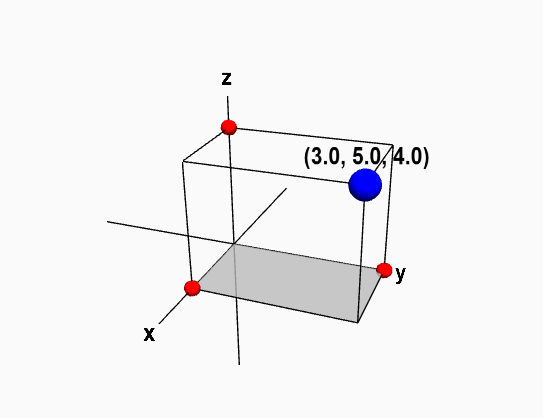
\includegraphics[scale=0.5]{cartesian coordinate 3d.png}
  \caption[Cartesian coordinate]{ตัวอย่างจุดบนระบบพิกัดคาร์ทีเซียนสามมิติ}
  \label{fig:cartesian}
\end{figure}
ซึ่งในการสร้างเกมเราจำเป็นต้องระบุตำแหน่งต่างๆของ GameObject ดังนั้นการสร้างเกมใน Unity จึงจำเป็นต้องรู้จักกับระบบพิกัดคาร์ทีเซียนสามมิติด้วย


\section{State Machine}
\enskip \enskip \enskip \enskip \enskip คือ การทำงานแบบมีการเปลี่ยนสถานะการทำงาน(state)ไปเรื่อยๆ เป็นขั้นตอนๆอย่างชัดเจน ซึ่งเป็นการมองสถานะการทำงานต่างๆ
เป็น state โดยที่เมื่อ input เข้ามาก็จะมีการเปลี่ยนสถานะการทำงาน(เปลี่ยนไป state ใหม่) หรืออาจจะไม่เปลี่ยนก็(อยู่ที่ state เดิม)ได้ขึ้นกับ input ซึ่งการจะเปลี่ยนสถานะแต่ละครั้ง
ขึ้นกับหลายๆอย่าง ได้แก่สถานะปัจจุบัน input เงือนไขต่างๆที่มีผลต่อการเปลี่ยนสถานะ ตัวอย่าง state machine เช่น ระบบประตูอัตโนมัติ โดยจะมีอยู่สอง state คือ ปิด และเปิด 
โดยเมื่อถ้าประอยู่ state "ปิด" แล้วมี input คือ มีคนอยู่หน้าประตู หลังจากได้รับ input ประตูก็จะเปลี่ยน state ไปเป็น "เปิด" ซึ่งถ้าไม่มีคนเเล้วประตูก็จะเปลี่ยน state เป็น "ปิด"
ซึ่งในการสร้างเกมมีการนำ state machine เข้ามาใช้ในการแสดง animation ต่างๆ ไม่ว่าจะเป็น การเดิน การวิ่ง การกระโดด โจมตี และอื่นๆ
% \begin{center}
% 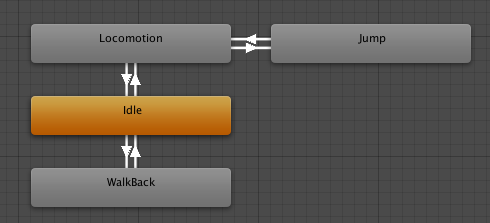
\includegraphics[scale=0.6]{MecanimStateMachine.png}
% \end{center}
% \begin{center}
% รูปที่ 2.2: ตัวอย่าง State Machine ที่ใช้ควบคุม animation
% \end{center}
% \graphicspath{ {./images/} }

\begin{figure}[htbp]
  \centering 
  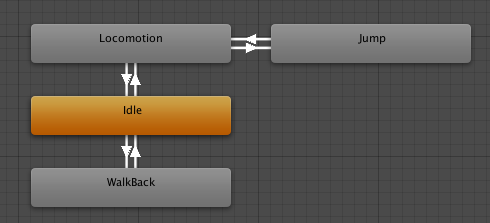
\includegraphics[scale=0.6]{MecanimStateMachine.png}
  \caption[State Machine]{ตัวอย่าง State Machine ที่ใช้ควบคุม animation}
  \label{fig:stateMachine}
\end{figure}

\section{ภาษา \texttt{C\#}}
\enskip \enskip \enskip \enskip \enskip เป็นภาษาคอมพิวเตอร์ที่เขียนโปรแกรมแบบ multi-paradigm~\cite{multiParadigm} โดยมีรูปแบบกฎเกณฑ์ และ
ข้อบังคับในการเขียนที่เข้มงวด ซึ่งมีคุณสมบัติในการเขียนแบบ function เหมือนกับการเขียนภาษาทั่วไป และเป็นการเขียนโปรแกรมแบบ OOP โดย \texttt{C\#} ถูกพัฒนาโดย 
Microsoft ภายใต้ .NET Framework~\cite{NET_Framework} โดยในการพัฒนาภาษา \texttt{C\#} นี้ มีความตั้งใจให้เป็นภาษาที่เขียนง่าย ทันสมัย 

\enskip \enskip \enskip ใน Unity ภาษา \texttt{C\#} ถูกนำมาใช้เป็นภาษาหลักในการเขียน script หรือ code ที่ทำหน้าที่จัดการกับการทำงานต่างๆในเกม
โดยรองรับหลากหลาย Framework เช่น Visual studio, VS code เป็นต้น

% \subsubsection{Subsubsection 1 heading goes here}
% Subsubsection 1 text

% \subsubsection{Subsubsection 2 heading goes here}
% Subsubsection 2 text

% \section{Third section}
% Section 3 text. The dielectric constant\index{dielectric constant}
% at the air-metal interface determines
% the resonance shift\index{resonance shift} as absorption or capture occurs
% is shown in Equation~\eqref{eq:dielectric}:

% \begin{equation}\label{eq:dielectric}
% k_1=\frac{\omega}{c({1/\varepsilon_m + 1/\varepsilon_i})^{1/2}}=k_2=\frac{\omega
% \sin(\theta)\varepsilon_\mathit{air}^{1/2}}{c}
% \end{equation}

% \noindent
% where $\omega$ is the frequency of the plasmon, $c$ is the speed of
% light, $\varepsilon_m$ is the dielectric constant of the metal,
% $\varepsilon_i$ is the dielectric constant of neighboring insulator,
% and $\varepsilon_\mathit{air}$ is the dielectric constant of air.

% \section{About using figures in your report}

% define a command that produces some filler text, the lorem ipsum.
% \newcommand{\loremipsum}{
%   \textit{Lorem ipsum dolor sit amet, consectetur adipisicing elit, sed do
%   eiusmod tempor incididunt ut labore et dolore magna aliqua. Ut enim ad
%   minim veniam, quis nostrud exercitation ullamco laboris nisi ut
%   aliquip ex ea commodo consequat. Duis aute irure dolor in
%   reprehenderit in voluptate velit esse cillum dolore eu fugiat nulla
%   pariatur. Excepteur sint occaecat cupidatat non proident, sunt in
%   culpa qui officia deserunt mollit anim id est laborum.}\par}

% \begin{figure}
%   \centering

%   \fbox{
%      \parbox{.6\textwidth}{\loremipsum}
%   }

%   % To include an image in the figure, say myimage.pdf, you could use
%   % the following code. Look up the documentation for the package
%   % graphicx for more information.
%   % \includegraphics[width=\textwidth]{myimage}

%   \caption[Sample figure]{This figure is a sample containing \gls{lorem ipsum},
%   showing you how you can include figures and glossary in your report.
%   You can specify a shorter caption that will appear in the List of Figures.}
%   \label{fig:sample-figure}
% \end{figure}

% Using \verb.\label. and \verb.\ref. commands allows us to refer to
% figures easily. If we can refer to Figures
% \ref{fig:walrus} and \ref{fig:sample-figure} by name in the {\LaTeX}
% source code, then we will not need to update the code that refers to it
% even if the placement or ordering of the figures changes.

% \loremipsum\loremipsum

% % This code demonstrates how to get a landscape table or figure. It
% % uses the package lscape to turn everything but the page number into
% % landscape orientation. Everything should be included within an
% % \afterpage{ .... } to avoid causing a page break too early.
% \afterpage{
%   \begin{landscape}
%   \begin{table}
%     \caption{Sample landscape table}
%     \label{tab:sample-table}

%     \centering

%     \begin{tabular}{c||c|c}
%         Year & A & B \\
%         \hline\hline
%         1989 & 12 & 23 \\
%         1990 & 4 & 9 \\
%         1991 & 3 & 6 \\
%     \end{tabular}
%   \end{table}
%   \end{landscape}
% }

% \loremipsum\loremipsum\loremipsum

% \section{Overfull hbox}

% When the \verb.semifinal. option is passed to the \verb.cpecmu. document class,
% any line that is longer than the line width, i.e., an overfull hbox, will be
% highlighted with a black solid rule:
% \begin{center}
% \begin{minipage}{2em}
% juxtaposition
% \end{minipage}
% \end{center}

\section{\ifenglish%
\ifcpe CPE \else ISNE \fi knowledge used, applied, or integrated in this project
\else%
ความรู้ตามหลักสูตรซึ่งถูกนำมาใช้หรือบูรณาการในโครงงาน
\fi
}
\enskip \enskip \enskip \enskip \enskip ในการทำโครงงานนี้กลุ่มของพวกเราได้นำความรู้ตามหลักสูตรต่างๆ มาประยุกต์ใช้ ซึ่งได้แก่
\subsection{ความรู้ที่ได้จากหลักสูตรวิชา Object Oriented Programming 261200}
\begin{enumerate}
\item การเขียนโปรแกรมเชิงวัตถุ(Object Oriented Programming : OOP) โดยการเขียนโปรแกรมเชิงวัตถุ กลุ่มของพวกเราได้นำมาใช้ในการวางแผน โดยการสร้าง interface และเขียน script ควบคุมการทำงาน โดยจะมีการออกแบบระบบต่างๆในเกมเป็น class 
เช่น class ของ characterController ใช้ควบคุมการควบคุมตัวละครโดยรวม, Status ใช้ในการควบคุมสถานะต่างๆของตัวละคร, AttackPoint ใช้คำนวณ damage จากการต่อสู้ เป็นต้น 
\item การนำเอา design patterns มาใช้ในการเขียน code โดยในส่วนที่ต้องการให้ object ใดๆมีเพียงแค่ตัวเดียวได้มีการนำ Singleton มาใช้ เพื่อป้องการทำงานซ้ำซ้อนของ code, ในส่วน
ที่เป็นการคำนวณ damage ซึ่งการ damage มีอยู่หลากหลายรูปแบบ เช่น damage จากการโจมตีเเบบ 1 hit, damage จากการโจมตีเเบบต่อเนื่อง(ติดสถานะต่างๆ), damage จากการโจมตี magic attack เป็นต้น
ซึ่งเพื่อให้ code มีความยืดหยุ่นเมื่อมีการโจมตีรูปแบบใหม่เพิ่มเข้ามา จึงได้มีการใช้ Strategy เข้ามาช่วย ซึ่งจะทำการสร้าง interface รวมที่คอยจัดการเกี่ยวกับการคำนวณ damage ต่างๆไว้ที่เดียวกัน นอกจากนี้ยังมี
code ส่วนอื่นๆก็มีการนำ design patterns มาใช้เช่นกัน
\end{enumerate}

\subsection{ความรู้ที่ได้จากหลักสูตรวิชา Calculus III 206261}
\begin{enumerate}
\item การคำนวณทางปริมาณ vector โดยได้นำความรู้ต่างๆในเรื่อง calculus vector มาใช่ในการคำนวณต่างๆภายในเกม เช่น ทิศทางการเดิน, ทิศทางการโจมตี เป็นต้น 
รวมถึงการนำความรู้ทาง vector มาช่วยในการทำความเข้าใจการทำงานต่างๆของ method ต่างที่อยู่ใน Unity
\item ความเร็ว ความเร่ง โดยได้นำความรู้เรื่อง อัตราการเปลี่ยนแปลงของความเร็ว คือ ความเร่ง มาประยุกต์ใช้ในการหาความเร็วของวัตถุ
\end{enumerate}

\subsection{ความรู้ที่ได้จากหลักสูตรวิชา Data Structure 261217}
\enskip \enskip \enskip การเก็บข้อมูลในรูปแบบต่างๆ โดยใน Unity การเขียน script บางครั้งต้องมีการเก็บข้อมูลต่างๆในเกมที่มีลักษณะที่แตกต่างกันออกไป ซึ่งข้อมูลเหล่านี้
จะเหมาะกับการเก็บใน structure ต่างๆแตกต่างกันออกไป เช่น การเก็บของที่ตัวละครเก็บได้ ควรจะเก็บเป็นรูปแบบ key และ value โดย key เป็น ชื่อของสิ่งของ
ส่วน value คือ จำนวนของสิ่งของนั้นๆ เป็นต้น

\subsection{ความรู้ที่ได้จากหลักสูตรวิชา ฟิสิกส์ 1 207105}
\begin{enumerate}
\item ปริมาณทางฟิสิกส์ โดยในการสร้างเกม ระบบของเกมจะอิงตามหลักความเป็นจริง ซึ่งได้มีการใช้ปริมาณทางฟิสิกส์ต่างๆ เช่น ความเร็ว, ความเร่ง, 
แรงเสียดทาน, แรงโน้มถ่วง, มวล เป็นต้น
\item การเคลื่อนที่ต่างๆ มีการเคลื่อนที่หลากหลายรูปแบบที่สามารถเกิดขึ้นภายในเกมได้ เช่น การเคลื่อนที่ในแนวดิ่ง, การเคลื่อนที่วิถีโค้ง(projectile), การเคลื่อนที่แบบมีแรงเสียดทานต่างๆ เป็นต้น
\end{enumerate}

\subsection{ความรู้ที่ได้จากหลักสูตรวิชา discrete mathematics 261216}
\begin{enumerate}
\item state machine โดยใช้ในการควบคุมการทำงานของ animation ของตัวละครต่างๆภาายในเกม
\item ความรู้ทางด้านตรรกศาสตร์ ใช้ในการออกแบบ เงื่อนไขต่างๆภายในเกม
\end{enumerate}



% อธิบายถึงความรู้ และแนวทางการนำความรู้ต่างๆ ที่ได้เรียนตามหลักสูตร ซึ่งถูกนำมาใช้ในโครงงาน

\section{\ifenglish%
Extracurricular knowledge used, applied, or integrated in this project
\else%
ความรู้นอกหลักสูตรซึ่งถูกนำมาใช้หรือบูรณาการในโครงงาน
\fi
}
\enskip \enskip \enskip \enskip \enskip ในการทำโครงงานนี้กลุ่มของพวกเราได้นำความรู้นอกหลักสูตรต่างๆ มาประยุกต์ใช้ ซึ่งได้แก่

\subsection{ความรู้ทางด้านการสร้างเกมโดยใช้ Unity}
\enskip \enskip \enskip เนื่องจากเกมของกลุ่มพวกเราใช้ Unity ในการพัฒนา ดังนั้นจึงได้มีการศึกษาการใช้งาน function ส่วนประกอบต่างๆใน
Unity ดังที่กล่าวไว้ในข้อ 2.1 พื้นฐาน Unity และได้มีการไปศึกษาในส่วนของ VFX หรือ Visual effect เพื่อนำมาปรับใช้กับตัวเกมหลัก  

\subsection{ความรู้ทางด้านการเขียนภาษา \texttt{C\#}}
\enskip \enskip \enskip เนื่องจากเกมของกลุ่มพวกเราใช้ Unity ในการพัฒนา ซึ่งใช้ภาษา \texttt{C\#} ในการเขียน script กลุ่มของพวกเราจึงได้ทำการศึกษาเพิ่มเติมกันเอง
โดยอาศัยสื่อต่างๆทางอินเตอร์เน็ต เช่น youtube, unimy, google เป็นต้น ดังที่กล่าวไว้ในข้อ 2.7 ภาษา \texttt{C\#}

\subsection{ความรู้ทางด้านการปั้น Model โดยใช้ Blender}
\enskip \enskip \enskip เนื่องจากมาจากมี asset บางอย่างที่จำเป็นต้องมีในเกม แต่ asset เหล่านั่นไม่สามารถหาซื้อได้ หรือมีราคาแพงจนเกินไป หรือไม่มีขาย 
จึงจำเป็นที่จะต้องปั้น Model ขึ้นมาใช้เอง เช่น ถังน้ำ, ก้อนหิน, บันได เป็นต้น

\enskip \enskip \enskip และในบางครั้ง Model ที่ซื้อมามี shader ที่ไม่ต้องการ หรืออยากปรับ shader ให้เป็นรูปแบบที่ต้องการ จึงต้องใช้ Blender ช่วยในการ
จัดการกับประเด็นเหล่านี้ ดังที่กล่าวไว้ในข้อ 2.2 พื้นฐาน Blender



% อธิบายถึงความรู้ต่างๆ ที่เรียนรู้ด้วยตนเอง และแนวทางการนำความรู้เหล่านั้นมาใช้ในโครงงาน
